\section{Finding 14 - Sudo Access on Less for User bluey}
%center under chapter title a one row table with 6 coloumns and no borders
\vspace*{-0,3cm}
\begin{center}
    \begin{tabular}{c c c c}
        \textbf{Classification:} & Privilige Escalation & \textbf{Severity:} & \textbf{\textcolor{red}{High}}  
        \end{tabular}
\end{center}
The user ”bluey” has sudo access to the less command for the file ”auth.log”.


\subsection*{Finding Impact}
This allows the user ”bluey” to execute the following command:
\begin{lstlisting}[language=bash]
plunder bluey [~]: sudo /usr/bin/less /var/log/auth.log
\end{lstlisting}
Within less the user can execute the following command:
\begin{lstlisting}[language=bash]
! /bin/bash
\end{lstlisting}
This opens a root shell on the system due to the sudo access without a password.


\subsection*{Finding Details}
Using the following command as the user ”bluey” shows which commands the user can execute with sudo access:
\begin{lstlisting}[language=bash]
plunder bluey [~]: sudo -l

User bluey may run the following commands on plunder:
(root) NOPASSWD: /usr/bin/less /var/log/auth.log
\end{lstlisting}

The Reason for this is the sudoers file:
\begin{figure}[h]
    \centering
    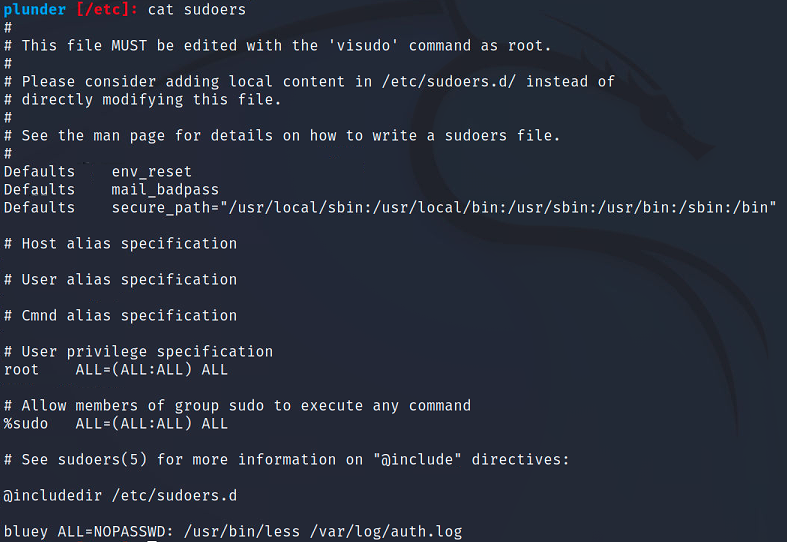
\includegraphics[width=1\textwidth]{img/sudoers_file.png}
    \caption{Sudoers File}
    \label{fig:fin14}
\end{figure}

The last line of this file gives the user ”bluey” sudo access to the less command for the file ”auth.log” without a password.

Exploting this vulnerability is shown in the following screenshot:
\begin{figure}[H]
    \centering
    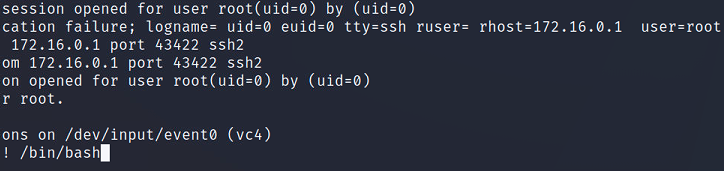
\includegraphics[width=1\textwidth]{img/less_exploit.png}
    \caption{Screenshot of Exploit}
    \label{fig:fin14-1}
\end{figure}
After executing this command the user ”bluey” has a root shell on the system.

\subsection*{Evaluation of Results}
\begin{center}
    \begin{tabular}{cccc}
    \textbf{Effort to Fix:} & &\ \textbf{\textcolor{green!50!blue}{Low}}\
    \end{tabular}
\end{center}
Remove the sudo access for the user ”bluey” in the sudoers file.
This can be done by using the following command:
\begin{lstlisting}[language=bash]
$ sudo visudo
\end{lstlisting}
And then removing the line:
\begin{lstlisting}[language=bash]
bluey ALL=NOPASSWD: /usr/bin/less /var/log/auth.log
\end{lstlisting}